% This is the Reed College LaTeX thesis template. Most of the work
% for the document class was done by Sam Noble (SN), as well as this
% template. Later comments etc. by Ben Salzberg (BTS). Additional
% restructuring and APA support by Jess Youngberg (JY).
% Your comments and suggestions are more than welcome; please email
% them to cus@reed.edu
%
% See http://web.reed.edu/cis/help/latex.html for help. There are a
% great bunch of help pages there, with notes on
% getting started, bibtex, etc. Go there and read it if you're not
% already familiar with LaTeX.
%
% Any line that starts with a percent symbol is a comment.
% They won't show up in the document, and are useful for notes
% to yourself and explaining commands.
% Commenting also removes a line from the document;
% very handy for troubleshooting problems. -BTS

% As far as I know, this follows the requirements laid out in
% the 2002-2003 Senior Handbook. Ask a librarian to check the
% document before binding. -SN

%%
%% Preamble
%%
% \documentclass{<something>} must begin each LaTeX document
\documentclass[12pt,twoside]{reedthesis}
% Packages are extensions to the basic LaTeX functions. Whatever you
% want to typeset, there is probably a package out there for it.
% Chemistry (chemtex), screenplays, you name it.
% Check out CTAN to see: http://www.ctan.org/
%%
\usepackage{graphicx,latexsym}
\usepackage{amsmath}
\usepackage{amssymb,amsthm}
\usepackage{longtable,booktabs,setspace}
\usepackage{chemarr} %% Useful for one reaction arrow, useless if you're not a chem major
\usepackage[hyphens]{url}
% Added by CII
\usepackage{hyperref}
\usepackage{lmodern}
\usepackage{float}
\floatplacement{figure}{H}
% End of CII addition
\usepackage{rotating}

% Next line commented out by CII
%%% \usepackage{natbib}
% Comment out the natbib line above and uncomment the following two lines to use the new
% biblatex-chicago style, for Chicago A. Also make some changes at the end where the
% bibliography is included.
%\usepackage{biblatex-chicago}
%\bibliography{thesis}


% Added by CII (Thanks, Hadley!)
% Use ref for internal links
\renewcommand{\hyperref}[2][???]{\autoref{#1}}
\def\chapterautorefname{Chapter}
\def\sectionautorefname{Section}
\def\subsectionautorefname{Subsection}
% End of CII addition

% Added by CII
\usepackage{caption}
\captionsetup{width=5in}
% End of CII addition

% \usepackage{times} % other fonts are available like times, bookman, charter, palatino

% Syntax highlighting #22

% To pass between YAML and LaTeX the dollar signs are added by CII
\title{Mean Estimation via Neural Network Methods in Complex Survey Imputation}
\author{Alexander Michael Moore}
% The month and year that you submit your FINAL draft TO THE LIBRARY (May or December)
\date{May 2019}
\division{Mathematics and Statistics}
\advisor{Kelly McConville}
\institution{Reed College}
\degree{Bachelor of Arts}
%If you have two advisors for some reason, you can use the following
% Uncommented out by CII
% End of CII addition

%%% Remember to use the correct department!
\department{Mathematics}
% if you're writing a thesis in an interdisciplinary major,
% uncomment the line below and change the text as appropriate.
% check the Senior Handbook if unsure.
%\thedivisionof{The Established Interdisciplinary Committee for}
% if you want the approval page to say "Approved for the Committee",
% uncomment the next line
%\approvedforthe{Committee}

% Added by CII
%%% Copied from knitr
%% maxwidth is the original width if it's less than linewidth
%% otherwise use linewidth (to make sure the graphics do not exceed the margin)
\makeatletter
\def\maxwidth{ %
  \ifdim\Gin@nat@width>\linewidth
    \linewidth
  \else
    \Gin@nat@width
  \fi
}
\makeatother

\renewcommand{\contentsname}{Table of Contents}
% End of CII addition

\setlength{\parskip}{0pt}

% Added by CII

\providecommand{\tightlist}{%
  \setlength{\itemsep}{0pt}\setlength{\parskip}{0pt}}

\Acknowledgements{
I want to thank a few people.
}

\Dedication{
You can have a dedication here if you wish.
}

\Preface{
This is an example of a thesis setup to use the reed thesis document
class (for LaTeX) and the R bookdown package, in general.
}

\Abstract{
Abstract last. 100-500 words. Abstract should be able to stand alone:
results and approach blatantly and simply stated. Want to sell paper at
a glimpse
\begin{itemize}
\tightlist
\item
  main objectiuve and rationale of project
\item
  outline of methods used
\item
  results of the project
\item
  conclusions about the implications of the project
\end{itemize}
}

% End of CII addition
%%
%% End Preamble
%%
%
\begin{document}

% Everything below added by CII
  \maketitle

\frontmatter % this stuff will be roman-numbered
\pagestyle{empty} % this removes page numbers from the frontmatter
  \begin{acknowledgements}
    I want to thank a few people.
  \end{acknowledgements}
  \begin{preface}
    This is an example of a thesis setup to use the reed thesis document
    class (for LaTeX) and the R bookdown package, in general.
  \end{preface}
  \hypersetup{linkcolor=black}
  \setcounter{tocdepth}{2}
  \tableofcontents

  \listoftables

  \listoffigures
  \begin{abstract}
    Abstract last. 100-500 words. Abstract should be able to stand alone:
    results and approach blatantly and simply stated. Want to sell paper at
    a glimpse
    \begin{itemize}
    \tightlist
    \item
      main objectiuve and rationale of project
    \item
      outline of methods used
    \item
      results of the project
    \item
      conclusions about the implications of the project
    \end{itemize}
  \end{abstract}
  \begin{dedication}
    You can have a dedication here if you wish.
  \end{dedication}
\mainmatter % here the regular arabic numbering starts
\pagestyle{fancyplain} % turns page numbering back on

\chapter{Delete line 6 if you only have one
advisor}\label{delete-line-6-if-you-only-have-one-advisor}

Placeholder

\chapter{Complex Surveys}\label{complex-surveys}

Placeholder

\section{Survey Statistics}\label{survey-statistics}

\section{Imputation}\label{imputation}

\chapter{Neural Networks}\label{math-sci}

\section{Introduction to Machine
Learning}\label{introduction-to-machine-learning}
\begin{quote}
From the advent of computation, there has been a drive towards
automation. (Goodfellow, Bengio, \& Courville, 2016)
\end{quote}
The capacity to derive patterns from raw data is known as machine
learning, a broad term for an extremely diverse collection of
algorithms. Machine learning flips the script on classical programming:
whereas classical programming takes rules and data to produce answers,
machine learning creates rules from data and answers by being ``trained
rather than explicitly programmed. It's presented with many examples
relevant to a task, and it finds a structure that derives rules for
automating the task'' (Chollet \& Allaire, 2018).

Machine learning is intended to elucidate or predict patterns in data.
These algorithms handle anything from linear regression for predicting a
numerical response based on a number of features, to clustering for
visualization and assignment of untaught observation classes. Machine
learning models are trained by minimizing error during exposure to
labelled ``training'' data with some underlying distribution and random
noise. After training, models are passed unlabelled ``test'' data to
predict the corresponding unknown class or value. Predictive
(supervised) machine learning algorithms seek to emulate and elucidate a
true unknown generative function from which the data were drawn.

For imputation purposes, our goal will be to accurately estimate missing
values by approximating the generative function from which they are
drawn. Generative functions are of the form \[
y = f(x_1, x_2, \dots, x_n) + \epsilon
\] where the true label \(y\) of the observation is a function of the
features \(x_1, ..., x_n\) perturbed by some random noise \(\epsilon\).

The estimating model will be trained via exposure to labelled
observations, called the training data, then used to predict
observations with missing labels, called testing data. The challenge in
machine learning is learning the correct amount from training data in
order to derive the underlying distribution of the observations without
simply memorizing the labels of the training set. This memorizaion
problem is called overfitting and is central to machine learning.

\ref{fig:overfit} is an illustration of this pervasive principle in a
regression example. An overfit (or too-flexible) model simply learns the
observation's labels, rather than the underlying distribution (or
generative function, in this case a second-degree polynomial). The
overfit model fails to learn the underlying generative function, and
instead learns the random noise of the training observations, and thus
is a poor explanation of a new realization from the same generative
function, seen in \ref{fig:overfit} and \ref{fig:overfitre}:
\begin{figure}
\centering
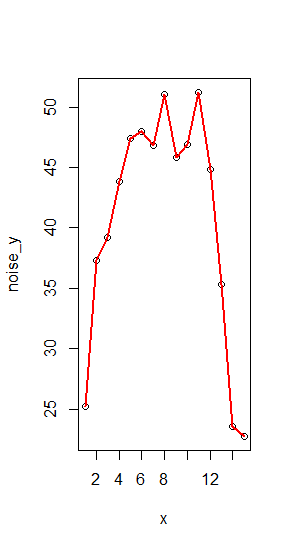
\includegraphics{figure/overfit.png}
\caption{\label{fig:overfit}The overfit model has extremely low error on the
realization of the data on which it was trained.}
\end{figure}
\begin{figure}
\centering
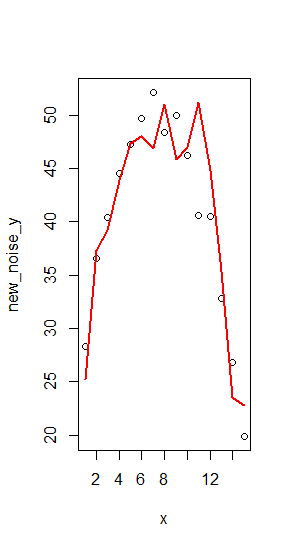
\includegraphics{figure/badfit.png}
\caption{\label{fig:overfitre}The overfit model does not accurately reflect
the underlying distribution from which both datasets are drawn. Rather,
it captures only the random noise of the data on which it was trained.
It would be a mistake to assume the generative function is a degree 15
polynomial just because the training error of such a function is low.}
\end{figure}
An underfit model, \ref{fig:underfit}, also fails to capture the
underlying distribution, due to a lack of flexibility. A linear
regression, though it minimizes its training MSE, clearly fails to
capture the underlying distribution of the data:
\begin{figure}
\centering
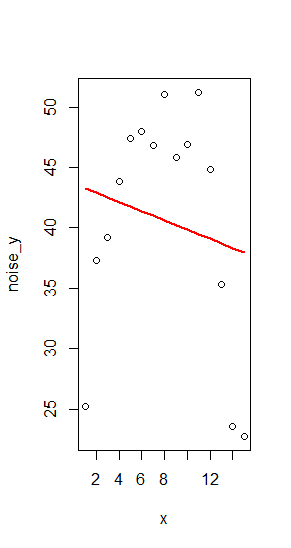
\includegraphics{figure/underfit.png}
\caption{\label{fig:underfit}An underfit model fails to capture the
underlying distribution}
\end{figure}
\ref{fig:goodmod} displays a well-trained model which straddles these
extrema and captures the apparent underlying distribution of the data in
a general sense by approximating the generative function from which they
are drawn, and remains fairly constant under different draws from the
same distribution. The aptly-flexible model has consistent performance
on new realizations of the data. The model performing well on data it
was not trained on is called generalizability.

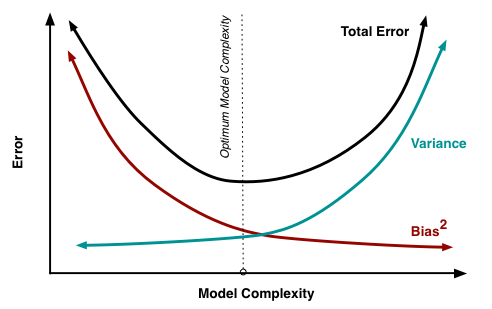
\includegraphics{figure/biasvariance.png} Fortmann, Scott. ``Bias and
Variance.'' Understanding the Bias-Variance Tradeoff, June 2012,
scott.fortmann-roe.com/docs/BiasVariance.html.

Figure \ref{fig:biasvar} demonstrates the involvement of model
complexity (or flexibility) in terms of training error. Model complexity
refers to the ability of the model to approximate complex generative
functions. We see that as the flexibility of the model increases, the
bias on the training set always decreases, representing the model's
performance on observations with labels. However, complexity beyond the
models optimal value implies over-flexibility, in which the model is
able to memorize random noise rather than stopping at the trend of the
data. This increases the total error of the model when exposed to data
that comes from the same generative function that the model has not been
exposed to, such as a testing data set or another observation from
outside the training set. Higher flexibility models create more variable
models, which though trained on data from the same generative function
differ greatly in appearance due to the random sample of training data.
These models are unstable for inference and generalize poorly.

One key difference from statistical modelling and survey statistics
methods is the point at which randomness is introduced into the data.
Machine learning attempts to approximate the function from which the
data was randomly generated, while survey statistics imply that
randomness in data comes from the survey design. The paradox of where
randomness is introduced into the data is resolved with the existence of
a superpopulation \(U\), where each observation has label
\(y = f(x) + \epsilon\), some generative function. From this
superpopulation, a population \(u\) is created through \emph{i.i.d.}
realizations from \(U\). From this population \(u\), the survey is
taken. Thus there still exists a generative function from which the
population is drawn, but the features and label of the observations are
fixed by the time the complex survey is taken on the population,
reconciling the two methodologies.

\section{Neural Networks}\label{neural-networks}

\subsection{Background and Context}\label{background-and-context}

Neural networks are a family of machine learning algorithms with an
extended and diverse history of research in neuroscience, statistics,
and computer science. Recently, these models have experienced great
growth in attention and popularity due to the contemporary circumstance
of computational capability. Neural networks thrive on large training
data sets, which have tended to increase in size and availability
throughout time. Neural networks also outperform competing algorithms in
high-dimension feature problems, which are common in real-world machine
learning applications such as image data, waveform data, and large
surveys. Often utilizing derivatives of complex compositions of
functions as an optimization method, deep learning training periods are
computationally intensive, relying heavily on computer hardware and
optimized software for reasonable implementation. Lastly, recent
attention to and development of neural networks can be attributed to
their proven potential in solving complicated real-world applications
with promising and increasingly dominant accuracy in practice, often at
the cost of a lack of inferability.

This lack of inferability is the typical downside of working with neural
networks as the inference on a model can be more important than the
predictive accuracy depending on the problem. Once a simple linear
regression is trained, the coefficients on the predictors offer an
immediately understandable interpretation of the behavior of the data.
For example, a coefficient of .3 on a feature \(x\) has a simple,
instant understanding: as feature \(x\) goes up by 1, the response goes
up by .3. Neural networks however, lack this instant recognition due to
the less intuitive layered structure of input transformations, known as
representation learning.

\subsection{Basics}\label{basics}

Neural Networks are a composition of functions. The following describes
a full neural network:

\[
\hat y = f(\boldsymbol{x}; \theta, \omega) = f^n ( f^{n-1}  ( ... f^1(\boldsymbol{x}; \theta, \omega)))
\] In this function, we see the input features \(x \in \mathbb{R}^n\),
the learned coefficients \(\theta\), the learning rate
\(\omega \in \mathbb{R}\), and the output prediction \(\hat{y}\).
Consider one of the layers of the network, \(f^i\). This layer is an
activation function composed with a linear function:

\[
f^i = \max ( 0 , {\boldsymbol{W}_i}^T \boldsymbol{x} + c_i)
\] Where \(\boldsymbol{W}_i^T \boldsymbol{x} + c_i\) is the interior
linear function for \(\boldsymbol{W}_i^T \in \mathbb{R}^n\),
\(c_i \in \mathbb{R}\).

The activation function shown above is the rectified linear unit, or
\(\max(0,a)\). Activation functions are significant as they introduce
nonlinearity into what would otherwise be a linear function (a
composition of linear functions). \({W_i}^T\) and \(c\) in \(f_i\)
dictate a linear transformation on the input to the layer. An ordered
list of all elements of \(W_i\) and \(c_i\) for all \(i \in n\) would
give the full description of the network, called \(\theta\). So the
output of a 1-layer network can be expressed as

\[
f(x; W, c, w, b) = w^T \max( 0 , \boldsymbol{W}^T \boldsymbol{x} +c ) +b
\]

The final activation function is another structural parameter left to
the designer of the network, but differs from interior activation
functions as the output of the network is restricted to the codomain of
the function, limiting the number of reasonable choices. The typical
output layer for scalar regression is a linear unit, on behalf of the
codomain \((-\infty,\infty)\) of the activation: \[
f^n(\boldsymbol{x}) = 1*(\boldsymbol{W}_n^T \boldsymbol{x} + c_n)
\]

The learning rate \(\omega\) and a loss function are meta-parameters,
given by the user creating the neural network. These two parameters are
used during the training of the network. During training, gradient
descent is used to descend the loss function in order to find the
optimal parameters for the network.

Loss functions are ways of describing the performance of a model when
predicting labels of a data set. The loss function takes the model and
data as inputs, and outputs a real number. Loss functions can be
minimized in training by optimization which leads the network to find
improvements in weights yielding accurate predictions. Loss functions
allow for another degree of customization in the training of a network,
such as in Ridge and LASSO regression. These algorithms add a weighting
to the typical mean squared error loss function which penalizes the
weights on predictors in polynomial regression. These methods introduce
bias into otherwise unbiased algorithms, but reduce the variability of
the model across different draws of data from the same distribution,
aiming to reduce the real test loss and improve the model. The cross
entropy between the data distribution and the model distribution is the
typical choice (Goodfellow et al., 2016).

Cross Entropy: \[
\int_\chi P(x) \log Q (x) dr(x) = E_p [- \log Q]
\]

Take for example the Mean Squared Error cost function: \[
MSE = \frac{1}{n} \sum_{k=1}^n  (y - \hat y)
\]

MSE, a typical loss function for regression applications, takes the mean
squared difference of the predicted label \(\hat y\) and the true label
\(y\) of the observations.
\begin{figure}
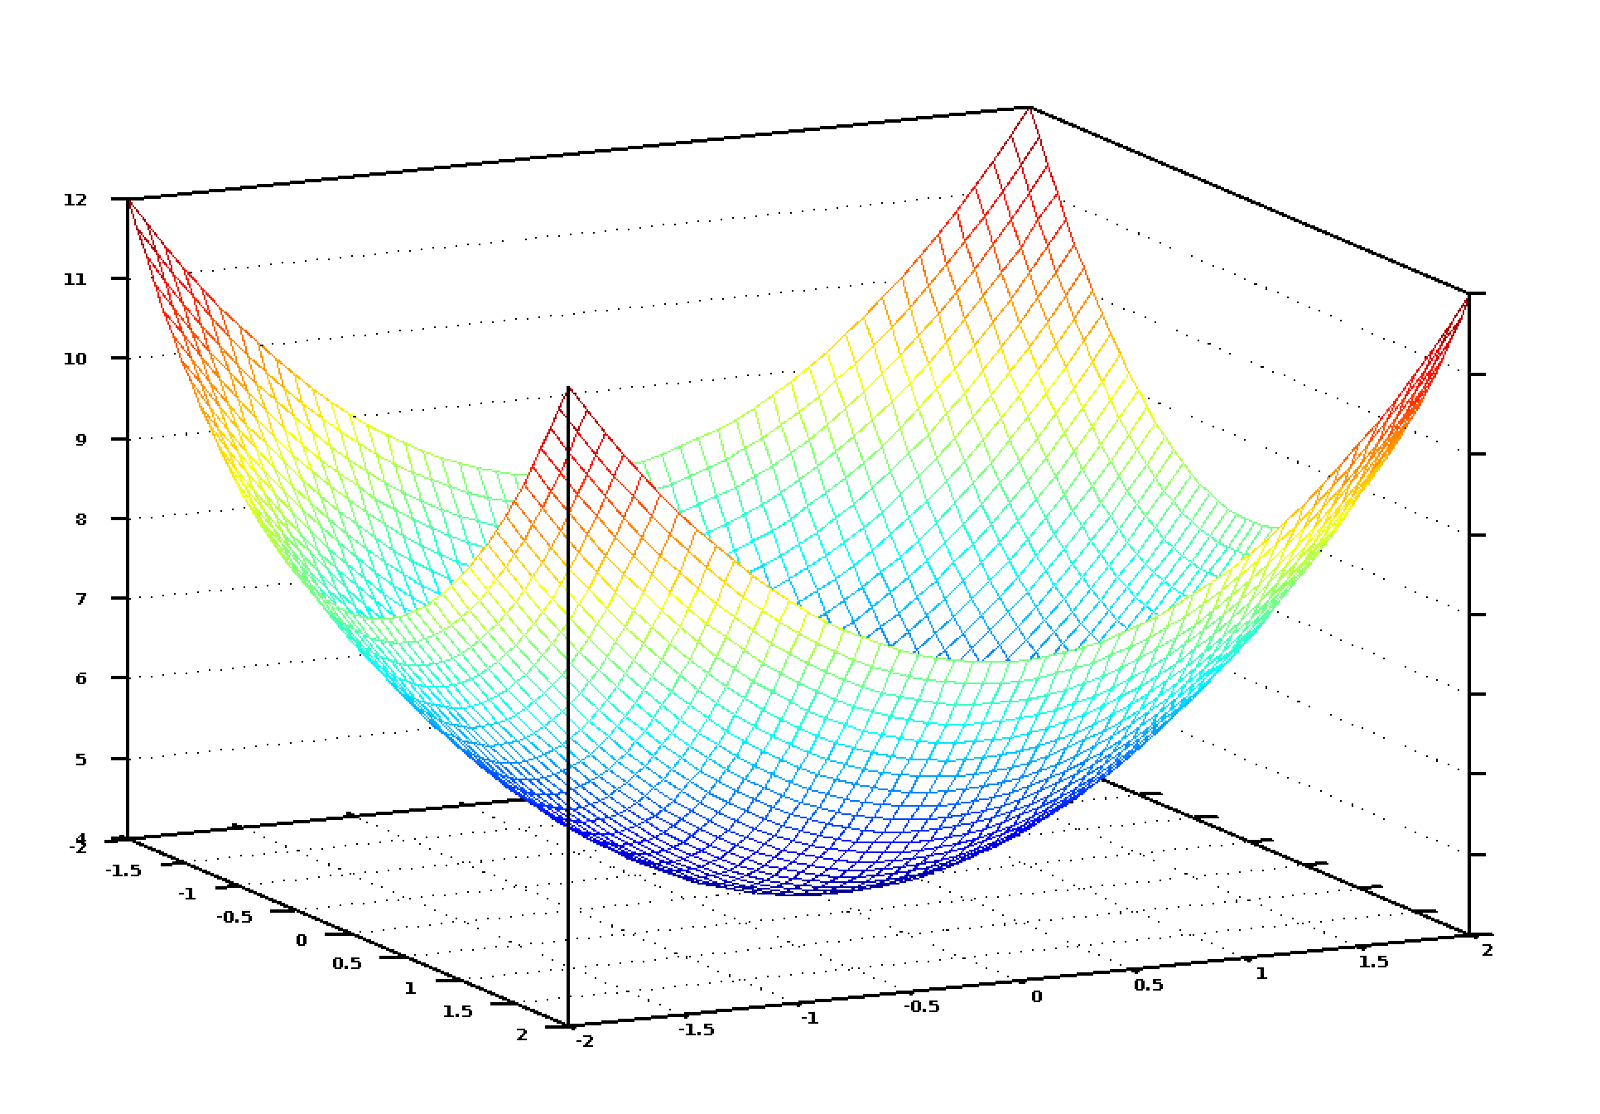
\includegraphics[width=0.4\linewidth]{figure/optimize} \caption{A convex loss function}\label{fig:optimize}
\end{figure}
\url{https://medium.com/@ageitgey/machine-learning-is-fun-80ea3ec3c471}

CITE ME

We can see that the loss of a linear regression is a function of \(m\)
and \(c\) given some data which is minimized at \(m = 0\) and \(c = 0\).
The learning rate is the amount that the functions' coefficients are
updated as the loss function is optimized from some initial coordinates
in search of the minimum loss.

Much like training a linear regression, the training of the neural
network aims to drive the approximating function to the underlying
function. The important difference induced by nonparametric models,
however, is the nonconvexity of the loss. The large amount of
coefficients which define even a relatively small network complicate the
optimization problem and make local minima a demanding distraction.
Optimization is typically done with gradient learning using a loss
function, or maximum likelihood estimation. Most modern neural networks
are trained using maximum likelihood, in which the cost function is the
negative log-likelihood between the training data and model distribution
(Goodfellow et al., 2016).

\subsection{Representation Learning}\label{representation-learning}

{[}{[}kelly, tell me if i should just delete this cheesy
paragraph:{]}{]} If you were handed a photograph and were asked if it
contained a car, there's a good chance you would immediately know the
answer. But how are you coming to this conclusion? The human mind
recognizes patterns of the image it has seen before, like a round
bumper, a rectangular windshield, and a few circular tires with a
certain spatial relationship to come to the conclusion that there is, in
fact, a car in the photograph. It is this process of representation
learning that prompted early researchers {[}{[}Citation Needed{]}{]} to
create representation-based learning algorithms to extrapolate on
information in the same way as the human mind. The emulation of human
neural cells was the birth of deep learning, a class of machine learning
algorithms which takes its name from multiple layers of connected nodes
simulating a proposed structure of the neurons of the human mind.
Representation learning takes observation's features as a first layer
into a composition of functions, in which each layer (or function)
transforms the data according to a learned representation transformation
that the subsequent layer takes as an input. This composition allows for
complex relationships of features to be learned in increasingly
sophisticated ways, making neural networks ideal for large-dimensional
datasets. For large-dimensional features, such as in Consumer Spending
Data, images, or audio, these hierarchical representations (or layered
representations) are important for distilling human-like feature
extraction and iterative predictor space transformation. To achieve
hierarchical representation properties, subsequent layers understand
more complex functions of input variables as each layer transforms
inputs and optimizes weights and weight relationships that minimize the
overall loss of the network. As each layer receives the transformed
output of the previous layer, more complex relationships of features can
be derived.

Successive layers of the network learn representation transformations of
the data which lend themselves to increasingly accurate description by
linear regression and activation performed by the final layer, called
the output layer. This process of successive transformation learns
meaningful representations on which the output layer can be most
accurate. Since the full network does not have a single functional
representation, it is nonparametric. The flexibility and power of neural
networks in fields demanding domain knowledge is that they can
approximate any function, per the Universal Approximation Theorem
(Hornik et al., 1989; Cybenko, 1989). The theorem states that a
feedforward network with a linear output layer and at least one hidden
layer with any ``squashing'' activation function can approximate any
Borel measurable function from one finite-dimensional space to another
with any desired nonzero amount of error, provided that the network is
given enough hidden units. Thus the user decision required is the depth
and breadth of the network, optimized through validation set
meta-analysis.

Representation learning is extremely important to the broad promises of
neural networks in practice. The basis for this strength is that
subsequent layers of the network learn meaningful structures of the
input data associated with a lower loss score. Correlations of features
forming a functional relationship to the label which induce loss
function descent will be internalized by the composition of subsequent
functions. This property of representation learning is significant for
investigating the necessity of independent and identically distributed
data in deep learning algorithms. It could be the case that the
significance of the inclusion probability can be learned as a meaningful
feature, with no special tweaks or preprocessing necessary for the
algorithm. Data which require no special tweeks are extremely meaningful
as this circumvents the necessity of incorporating domain knowledge and
expertise in current imputation methods, which holds back expedient and
lightweight research.

These advantages of Hierarchical and Distributed Representation
transformation give neural networks huge advantages in accuracy and
fitting capability for data with a massive hypothesis space. A
hypothesis space is the space of all possible answers to a question.
Image classification, for instance, represents a hypothesis space of
pixels with unknown correlations that must be trained with label
relationships to determine the correct distillation of millions of
pixels to a most-likely class label. Thus the curse of dimensionality
common throughout machine learning is mitigated through this manifold
learning process.

Neural networks thrive on the interaction of many features, due to the
nature of representation learning which excels in covariate relations
and distilling information encoded between features. Popular modern
applications are image and waveform audio data, in which machine
learning problems become dominated by the Curse of Dimensionality. This
common machine learning problem arises when the amount of data is
insignificant when compared to the hypothesis space or feature space,
and there are sparse observations for some regions. Machine learning
needs many observations with each combination of values, but this
becomes quickly infeasible for data with thousands of features. The
peaking phenomena dictates that there is an optimal number of features
to describe the data before the curse of dimensionality creates
problematic sparsity and dominating observations with few neighbors .
Neural networks are known to resist this commonplace issue due to the
distributed learning property, wherein each node is sensitive to only
particular features.

Distributed representation is a powerful implicit component of neural
networks in which neurons divide feature space to better handle feature
interactions: suppose an image-recognition system could recognize cars,
trucks, and birds, as well as distinguish if these objects are red,
green, or blue. One way of representing these inputs could be to have a
separate neuron for each combination: red truck, red car, red bird, and
so on for nine independent neurons. Distributed representation, however,
could partition these workloads by having three neurons for color and
three for object type. In addition to reducing the number of neurons
required dimensionally, this also distributes the learning demands of
each neuron. The neuron describing redness is able to learn about
redness from any category, not one specific category as the red bird
neuron must (Goodfellow et al., 2016).

Neural networks approximate nonlinear functions by applying linear
models not to the features x, but to a transformed input, \(\phi(x)\),
where \(\phi\) is a nonlinear transformation. \(\phi\) provides a new,
more meaningful representation for \(x\). The question then is how to
choose the mapping \(\phi\):
\begin{enumerate}
\def\labelenumi{\arabic{enumi}.}
\item
  One option is to manually engineer \(\phi\). This takes a huge
  speciality of domain knowledge and practitioner specialization, with
  little transfer between domains. This was the dominant method before
  deep learning (Goodfellow et al., 2016).
\item
  The strategy of neural networks comes from the learning of \(\phi\).
  ``In this approach, we have a model y = f(x; theta, w) as specified in
  the neural network introduction. Due to the Universal Approximation
  Theorem, the nonparametric deep feedforward network can learn a
  functional approximation from the input to the desired output. This
  method sacrifices the training convexity of the other two, but
  benefits from the genericity of the specifications. The human user
  need only specify a general function family rather than exactly the
  correct function, but can still benefit from designing families of
  \(\phi(x; \theta)\) that they expect to be relevant (Goodfellow et
  al., 2016).
\end{enumerate}
The neural network approximates some true underlying function
\(f^*(p; \theta)\) of the predictors \(x\) to the output category,
\(y\), and learns the coefficients \(\theta\) of the series of linear
transformations composing the layers that result in the best function
approximation. The number of functions in the composition is the called
the depth of the model. Our model is called \(\hat f\), the generative
function it seeks to approximate is called \(f\). The outputs of our
model are \(\hat y\) ``guess at y'' and the true labels are \(y\).

\subsection{Neural Networks for Complex Survey
Data}\label{neural-networks-for-complex-survey-data}

From an optimist's perspective, the need for data preprocessing or
special conditions on the loss function for training the model would be
unnecessary: If learning the correlations and underlying distributions
associated with rare observations from complex survey design would truly
lower the network's loss, it should be learned and accounted for without
the need to perform special external transformations on the data to
``undo'' the effects of complex sample design. For this reason, it is
significant to compare the potentially superior results of a naive model
to one with superfluous data transformations done. A neural network
model with access to an informative \(\pi\) feature ideally would
approximate the function relating the inclusion probability and features
to labels, without the need for extreme domain knowledge and manual
feature engineering.

The optimism of nonparametric algorithms increases in tasks of minimal
domain knowledge and feature engineering capability. Ideally, using
heuristic meta-parameters defining a neural network model would be
enough to get reasonable predictive accuracy in conjunction with one of
the methods of Chapter 3. Per the Universal Approximation Theorem, any
underlying generative function is at worst approximated by a 2 layer
heuristic model, potentially improving upon other naive modeling
procedures such as a weighted linear regression. Additionally, in real
survey data the capacity to derive the significant features from a
high-dimensional space is a weakness of parametric model regression,
which is highly variable in the context of noisy parameters, explored in
Chapter 4.

\chapter{Methods}\label{methods}

Placeholder

\section{Mean Estimation Methods}\label{mean-estimation-methods}

\subsection{Naive Mean:}\label{naive-mean}

\subsection{Pi-Corrected Naive Mean:}\label{pi-corrected-naive-mean}

\subsection{Oracle Mean:}\label{oracle-mean}

\section{Imputation Methods}\label{imputation-methods}

\subsection{Imputation Mean Estimator:}\label{imputation-mean-estimator}

\subsection{Drop.NA}\label{drop.na}

\subsection{Median Imputation}\label{median-imputation}

\subsection{Weighted Linear Regression
Imputation}\label{weighted-linear-regression-imputation}

\subsection{Naive Neural Network
Imputation}\label{naive-neural-network-imputation}

\subsection{Weighted Loss Neural Network
Imputation}\label{weighted-loss-neural-network-imputation}

\subsection{\texorpdfstring{\(\pi\)-Feature Neural Network
Imputation}{\textbackslash{}pi-Feature Neural Network Imputation}}\label{pi-feature-neural-network-imputation}

\subsection{Weighted Resample Neural Network
Imputation}\label{weighted-resample-neural-network-imputation}

\subsection{Derived Feature Neural Network
Imputation}\label{derived-feature-neural-network-imputation}

\chapter{Simulation}\label{simulation}

Placeholder

\section{Exploration of Methods Using
Simulation}\label{exploration-of-methods-using-simulation}

\section{High-Dimension Simulation}\label{high-dimension-simulation}

\section{Monte Carlo Simulation}\label{monte-carlo-simulation}

\section{Creating a Simulated
Population}\label{creating-a-simulated-population}

\section{Results aaaaaaaaa}\label{results-aaaaaaaaa}

\section{Results}\label{results}

\chapter{Consumer Expenditure
Surveys}\label{consumer-expenditure-surveys}

\section{Data}\label{data}

The Consumer Expenditure (CE) Surveys provide data on ``expenditures,
income, and demographic characteristics of consumers in the United
States (cite CE
\url{https://www.bls.gov/cex/pumd-getting-started-guide.htm}). CE data
are collected by the Census Bureau for the Bureau of Labor Statistics
(BLS). The data are primary used to revise the relative importance of
goods and services in the market basket of the Consumer Price Index''.

The data will be the \texttt{fmli171x} survey data

\section{Procedure}\label{procedure}

The CE data method performance comparison will be performed in much the
same way as the simulated data method comparison.

The \texttt{fmli171x} survey data is first pre-processed to remove
features with large swathes of missingness. For this study, features
with more than 33\% missing values are dropped from the data set.
Features with missingness less than 33\% are then median-imputed, where
missing values are replaced with the median value of the feature. The
median in this case is used for reasons: it returns only reasonable
values, is uninformative, and does not rely on multiple imputation.

The label to be used is \texttt{FINCBTAX}, the financial income of the
response household before taxes. This label has no missingness as it is
BLS-derived (already imputed).

This process returns a complete-case data set of 6208 family samples
across 607 variables. There are 127 million households in the US.

The problem of assessing model performance in real-world data is the
paradox of missing labels: ideally, we would impute a missing label,
then learn the true value, and score the model accordingly. For this
data, we will again rely on Monte Carlo simulation to create a
distribution of population mean estimates (U.S. mean household income)
by inducing missingness in the known labels, imputing, and comparing
results via MSE to the true mean.

The following process is repeated a number of times to create a
distribution of mean estimates for each method: 1. Record the true
(sample) mean and Horvitz-Thompson mean estimate 2. Induce missingness
on 20\% of the labels, weighted to larger labels 3. Perform and record
each model's mean estimate + For the real data, a more accurate neural
network method is adopted in which each network undergoes two trainings:
the first finds the ideal train duration by overtraining on the training
data, the second re-trains the model to the validation minimum of the
first model. 4. The results are compared using MSE, oracle ratio, and
PRB.

The dimension of the neural networks has changed somewhat to account for
the new data. Still working on the specifics of this \#\# Results Not a
place to list findings. Rather, convince that what I did is correct,
worthy of study, and impactful. Be honest about the generalizability of
the work. If the findings are negative, take care to explain why the
results still matter (discussion of why linear regression is so dank at
mean estimation). Cast the negative result as a useful insight, rather
than a problem with the methodology

\chapter*{Conclusion}\label{conclusion}
\addcontentsline{toc}{chapter}{Conclusion}

Placeholder

\section{The End}\label{the-end}

\section{Discussion}\label{discussion}

\section{Conclusion}\label{conclusion-1}

\section{Future Work}\label{future-work}

\appendix

\chapter{The First Appendix}\label{the-first-appendix}

This first appendix includes all of the R chunks of code that were
hidden throughout the document (using the \texttt{include\ =\ FALSE}
chunk tag) to help with readibility and/or setup.

\textbf{In the main Rmd file}

\textbf{In Chapter \ref{ref-labels}:}

\chapter{The Second Appendix, for
Fun}\label{the-second-appendix-for-fun}

\chapter*{References}\label{references}
\addcontentsline{toc}{chapter}{References}

Placeholder

\hypertarget{refs}{}
\hypertarget{ref-chollet2018deep}{}
Chollet, F., \& Allaire, J. (2018). Deep learning with r. manning
publications.

\hypertarget{ref-goodfellow2016deep}{}
Goodfellow, I., Bengio, Y., \& Courville, A. (2016). \emph{Deep
learning}. MIT press.


% Index?

\end{document}
